% Options for packages loaded elsewhere
\PassOptionsToPackage{unicode}{hyperref}
\PassOptionsToPackage{hyphens}{url}
%
\documentclass[
]{article}
\usepackage{lmodern}
\usepackage{amssymb,amsmath}
\usepackage{ifxetex,ifluatex}
\ifnum 0\ifxetex 1\fi\ifluatex 1\fi=0 % if pdftex
  \usepackage[T1]{fontenc}
  \usepackage[utf8]{inputenc}
  \usepackage{textcomp} % provide euro and other symbols
\else % if luatex or xetex
  \usepackage{unicode-math}
  \defaultfontfeatures{Scale=MatchLowercase}
  \defaultfontfeatures[\rmfamily]{Ligatures=TeX,Scale=1}
\fi
% Use upquote if available, for straight quotes in verbatim environments
\IfFileExists{upquote.sty}{\usepackage{upquote}}{}
\IfFileExists{microtype.sty}{% use microtype if available
  \usepackage[]{microtype}
  \UseMicrotypeSet[protrusion]{basicmath} % disable protrusion for tt fonts
}{}
\makeatletter
\@ifundefined{KOMAClassName}{% if non-KOMA class
  \IfFileExists{parskip.sty}{%
    \usepackage{parskip}
  }{% else
    \setlength{\parindent}{0pt}
    \setlength{\parskip}{6pt plus 2pt minus 1pt}}
}{% if KOMA class
  \KOMAoptions{parskip=half}}
\makeatother
\usepackage{xcolor}
\IfFileExists{xurl.sty}{\usepackage{xurl}}{} % add URL line breaks if available
\IfFileExists{bookmark.sty}{\usepackage{bookmark}}{\usepackage{hyperref}}
\hypersetup{
  pdftitle={Early Ovarian Cancer},
  pdfauthor={Kevin Kremer},
  hidelinks,
  pdfcreator={LaTeX via pandoc}}
\urlstyle{same} % disable monospaced font for URLs
\usepackage[margin=1in]{geometry}
\usepackage{color}
\usepackage{fancyvrb}
\newcommand{\VerbBar}{|}
\newcommand{\VERB}{\Verb[commandchars=\\\{\}]}
\DefineVerbatimEnvironment{Highlighting}{Verbatim}{commandchars=\\\{\}}
% Add ',fontsize=\small' for more characters per line
\usepackage{framed}
\definecolor{shadecolor}{RGB}{248,248,248}
\newenvironment{Shaded}{\begin{snugshade}}{\end{snugshade}}
\newcommand{\AlertTok}[1]{\textcolor[rgb]{0.94,0.16,0.16}{#1}}
\newcommand{\AnnotationTok}[1]{\textcolor[rgb]{0.56,0.35,0.01}{\textbf{\textit{#1}}}}
\newcommand{\AttributeTok}[1]{\textcolor[rgb]{0.77,0.63,0.00}{#1}}
\newcommand{\BaseNTok}[1]{\textcolor[rgb]{0.00,0.00,0.81}{#1}}
\newcommand{\BuiltInTok}[1]{#1}
\newcommand{\CharTok}[1]{\textcolor[rgb]{0.31,0.60,0.02}{#1}}
\newcommand{\CommentTok}[1]{\textcolor[rgb]{0.56,0.35,0.01}{\textit{#1}}}
\newcommand{\CommentVarTok}[1]{\textcolor[rgb]{0.56,0.35,0.01}{\textbf{\textit{#1}}}}
\newcommand{\ConstantTok}[1]{\textcolor[rgb]{0.00,0.00,0.00}{#1}}
\newcommand{\ControlFlowTok}[1]{\textcolor[rgb]{0.13,0.29,0.53}{\textbf{#1}}}
\newcommand{\DataTypeTok}[1]{\textcolor[rgb]{0.13,0.29,0.53}{#1}}
\newcommand{\DecValTok}[1]{\textcolor[rgb]{0.00,0.00,0.81}{#1}}
\newcommand{\DocumentationTok}[1]{\textcolor[rgb]{0.56,0.35,0.01}{\textbf{\textit{#1}}}}
\newcommand{\ErrorTok}[1]{\textcolor[rgb]{0.64,0.00,0.00}{\textbf{#1}}}
\newcommand{\ExtensionTok}[1]{#1}
\newcommand{\FloatTok}[1]{\textcolor[rgb]{0.00,0.00,0.81}{#1}}
\newcommand{\FunctionTok}[1]{\textcolor[rgb]{0.00,0.00,0.00}{#1}}
\newcommand{\ImportTok}[1]{#1}
\newcommand{\InformationTok}[1]{\textcolor[rgb]{0.56,0.35,0.01}{\textbf{\textit{#1}}}}
\newcommand{\KeywordTok}[1]{\textcolor[rgb]{0.13,0.29,0.53}{\textbf{#1}}}
\newcommand{\NormalTok}[1]{#1}
\newcommand{\OperatorTok}[1]{\textcolor[rgb]{0.81,0.36,0.00}{\textbf{#1}}}
\newcommand{\OtherTok}[1]{\textcolor[rgb]{0.56,0.35,0.01}{#1}}
\newcommand{\PreprocessorTok}[1]{\textcolor[rgb]{0.56,0.35,0.01}{\textit{#1}}}
\newcommand{\RegionMarkerTok}[1]{#1}
\newcommand{\SpecialCharTok}[1]{\textcolor[rgb]{0.00,0.00,0.00}{#1}}
\newcommand{\SpecialStringTok}[1]{\textcolor[rgb]{0.31,0.60,0.02}{#1}}
\newcommand{\StringTok}[1]{\textcolor[rgb]{0.31,0.60,0.02}{#1}}
\newcommand{\VariableTok}[1]{\textcolor[rgb]{0.00,0.00,0.00}{#1}}
\newcommand{\VerbatimStringTok}[1]{\textcolor[rgb]{0.31,0.60,0.02}{#1}}
\newcommand{\WarningTok}[1]{\textcolor[rgb]{0.56,0.35,0.01}{\textbf{\textit{#1}}}}
\usepackage{graphicx,grffile}
\makeatletter
\def\maxwidth{\ifdim\Gin@nat@width>\linewidth\linewidth\else\Gin@nat@width\fi}
\def\maxheight{\ifdim\Gin@nat@height>\textheight\textheight\else\Gin@nat@height\fi}
\makeatother
% Scale images if necessary, so that they will not overflow the page
% margins by default, and it is still possible to overwrite the defaults
% using explicit options in \includegraphics[width, height, ...]{}
\setkeys{Gin}{width=\maxwidth,height=\maxheight,keepaspectratio}
% Set default figure placement to htbp
\makeatletter
\def\fps@figure{htbp}
\makeatother
\setlength{\emergencystretch}{3em} % prevent overfull lines
\providecommand{\tightlist}{%
  \setlength{\itemsep}{0pt}\setlength{\parskip}{0pt}}
\setcounter{secnumdepth}{-\maxdimen} % remove section numbering
\usepackage{booktabs}
\usepackage{longtable}
\usepackage{array}
\usepackage{multirow}
\usepackage{wrapfig}
\usepackage{float}
\usepackage{colortbl}
\usepackage{pdflscape}
\usepackage{tabu}
\usepackage{threeparttable}
\usepackage{threeparttablex}
\usepackage[normalem]{ulem}
\usepackage{makecell}

\title{Early Ovarian Cancer}
\author{Kevin Kremer}
\date{9/24/2020}

\begin{document}
\maketitle

\hypertarget{early-stage-high-grade-serous-ovarian-cancer}{%
\section{Early Stage High-Grade Serous Ovarian
Cancer}\label{early-stage-high-grade-serous-ovarian-cancer}}

\hypertarget{survival-based-on-race}{%
\subsection{Survival based on race}\label{survival-based-on-race}}

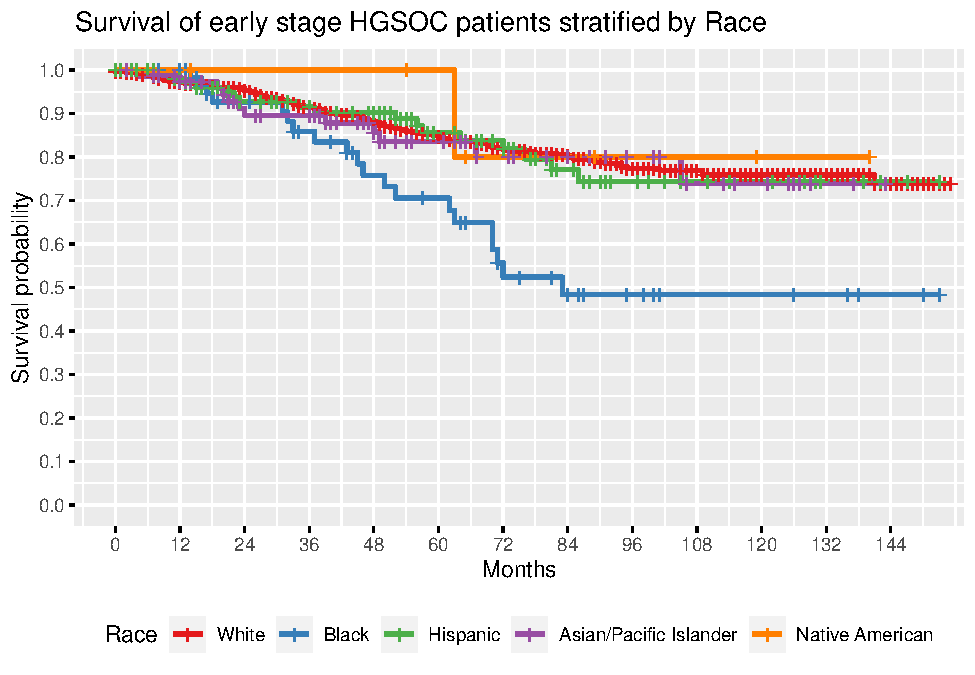
\includegraphics{EarlyOvaryByRace_files/figure-latex/unnamed-chunk-1-1.pdf}

\begin{Shaded}
\begin{Highlighting}[]
\KeywordTok{table}\NormalTok{(HGS}\OperatorTok{$}\NormalTok{Race)}
\end{Highlighting}
\end{Shaded}

\begin{verbatim}
## 
##    API  Black   Hisp Native    Unk  White 
##     94     73    137      7      3    956
\end{verbatim}

\hypertarget{comparing-black-race-to-all-other-races}{%
\subsection{Comparing Black Race to all other
races}\label{comparing-black-race-to-all-other-races}}

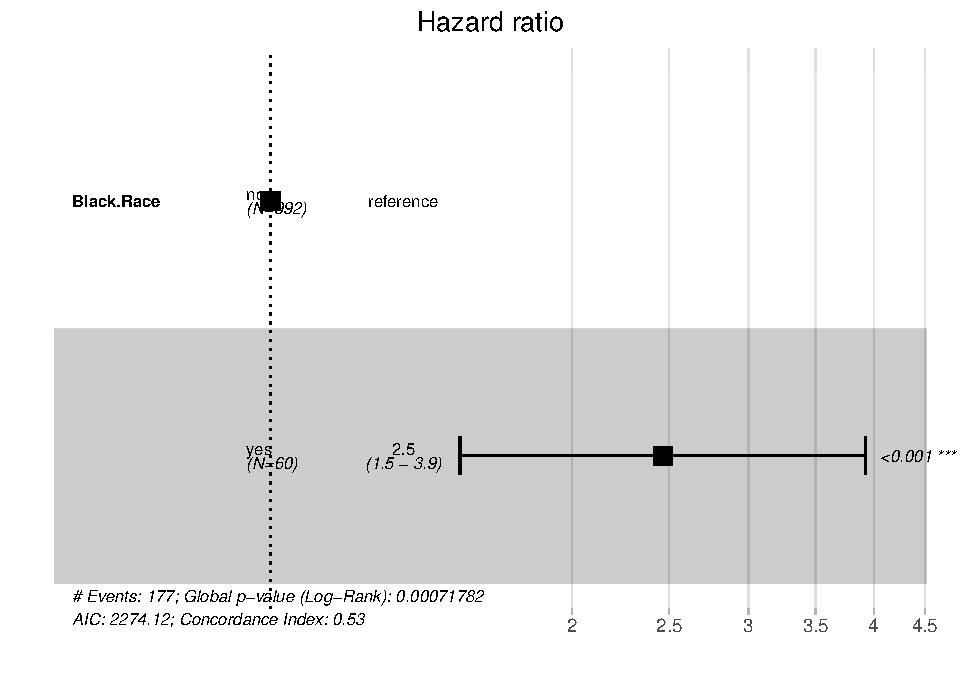
\includegraphics{EarlyOvaryByRace_files/figure-latex/unnamed-chunk-3-1.pdf}

\begin{Shaded}
\begin{Highlighting}[]
\NormalTok{HGS.tbl <-}\StringTok{ }\KeywordTok{table}\NormalTok{(HGS}\OperatorTok{$}\NormalTok{Black.Race)}
\KeywordTok{kbl}\NormalTok{(HGS.tbl, }\DataTypeTok{col.names =} \KeywordTok{c}\NormalTok{(}\StringTok{"Black Race"}\NormalTok{, }\StringTok{"Count"}\NormalTok{)) }\OperatorTok\StringTok{ }
\StringTok{        }\KeywordTok{kable_styling}\NormalTok{(}\DataTypeTok{bootstrap_options =} \StringTok{"striped"}\NormalTok{, }\DataTypeTok{full_width =}\NormalTok{ F, }\DataTypeTok{position =} \StringTok{"left"}\NormalTok{)}
\end{Highlighting}
\end{Shaded}

\begin{tabular}[t]{l|r}
\hline
Black Race & Count\\
\hline
no & 1197\\
\hline
yes & 73\\
\hline
\end{tabular}

\begin{Shaded}
\begin{Highlighting}[]
\NormalTok{HGS.chemo.tbl <-}\StringTok{ }\KeywordTok{table}\NormalTok{(HGS}\OperatorTok{$}\NormalTok{Black.Race, HGS}\OperatorTok{$}\NormalTok{Chemo) }
\KeywordTok{kbl}\NormalTok{(HGS.chemo.tbl) }\OperatorTok\StringTok{ }
\StringTok{        }\KeywordTok{kable_styling}\NormalTok{(}\DataTypeTok{bootstrap_options =} \StringTok{"striped"}\NormalTok{, }\DataTypeTok{full_width =}\NormalTok{ F, }\DataTypeTok{position =} \StringTok{"left"}\NormalTok{) }\OperatorTok\StringTok{ }
\StringTok{        }\KeywordTok{add_header_above}\NormalTok{(}\KeywordTok{c}\NormalTok{(}\StringTok{"Black Race"}\NormalTok{, }\StringTok{"Chemo Received"}\NormalTok{ =}\StringTok{ }\DecValTok{2}\NormalTok{))}
\end{Highlighting}
\end{Shaded}

\begin{tabular}[t]{l|r|r}
\hline
\multicolumn{1}{c|}{Black Race} & \multicolumn{2}{c}{Chemo Received} \\
\cline{1-1} \cline{2-3}
  & No/Unknown & Yes\\
\hline
no & 317 & 880\\
\hline
yes & 23 & 50\\
\hline
\end{tabular}

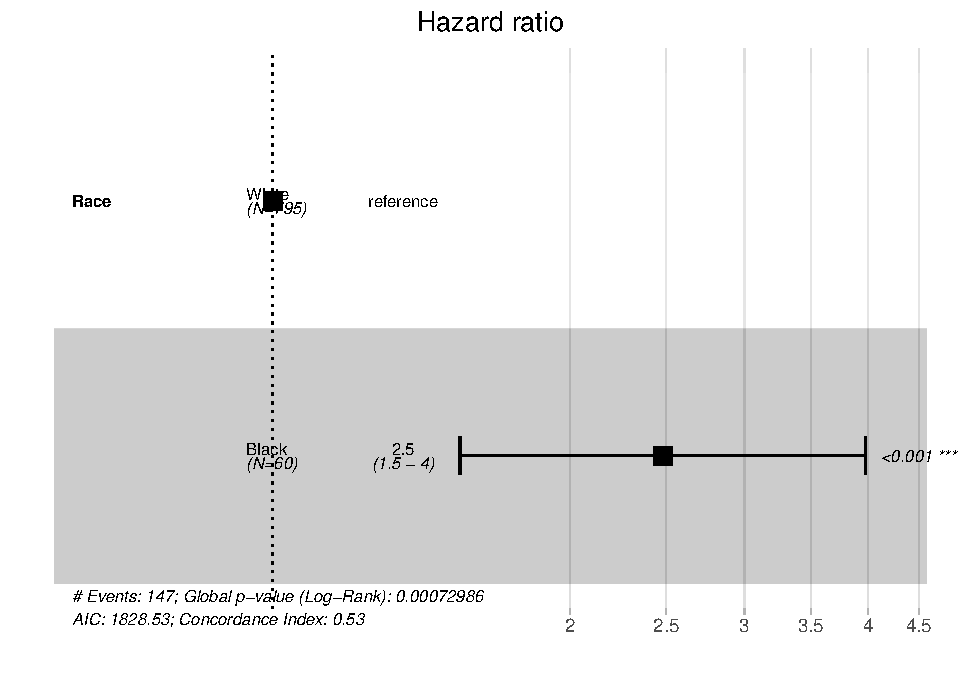
\includegraphics{EarlyOvaryByRace_files/figure-latex/unnamed-chunk-5-1.pdf}

\hypertarget{broken-down-by-stage}{%
\subsubsection{Broken down by Stage}\label{broken-down-by-stage}}

\hypertarget{t1n0m0}{%
\paragraph{T1N0M0}\label{t1n0m0}}

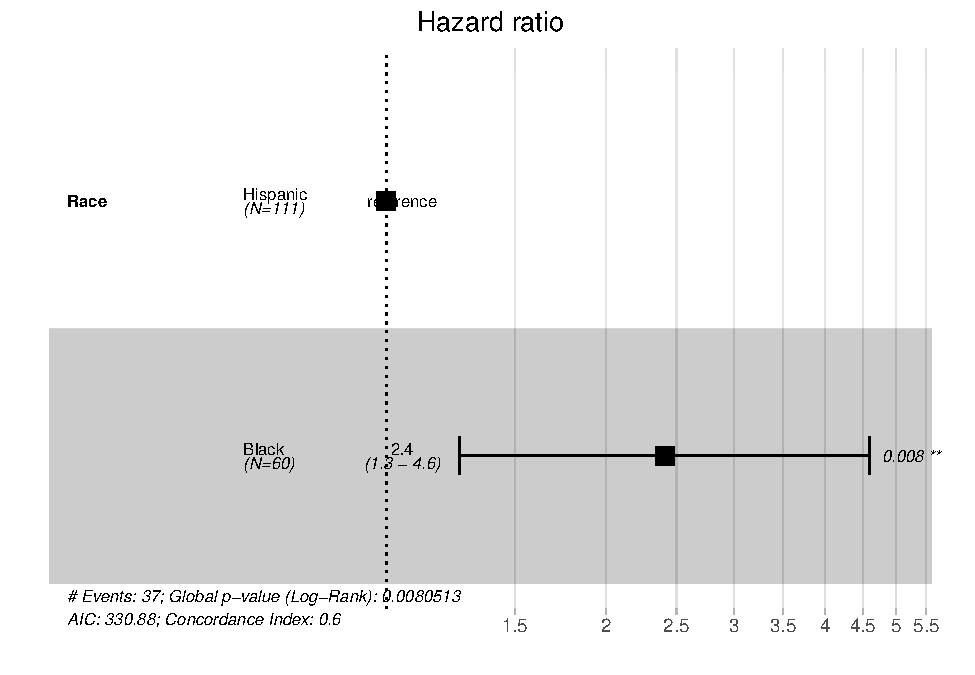
\includegraphics{EarlyOvaryByRace_files/figure-latex/unnamed-chunk-7-1.pdf}

\begin{Shaded}
\begin{Highlighting}[]
\KeywordTok{table}\NormalTok{(T1.N0.M0.Black}\OperatorTok{$}\NormalTok{Black.Race)}
\end{Highlighting}
\end{Shaded}

\begin{verbatim}
## 
##  no yes 
## 749  43
\end{verbatim}

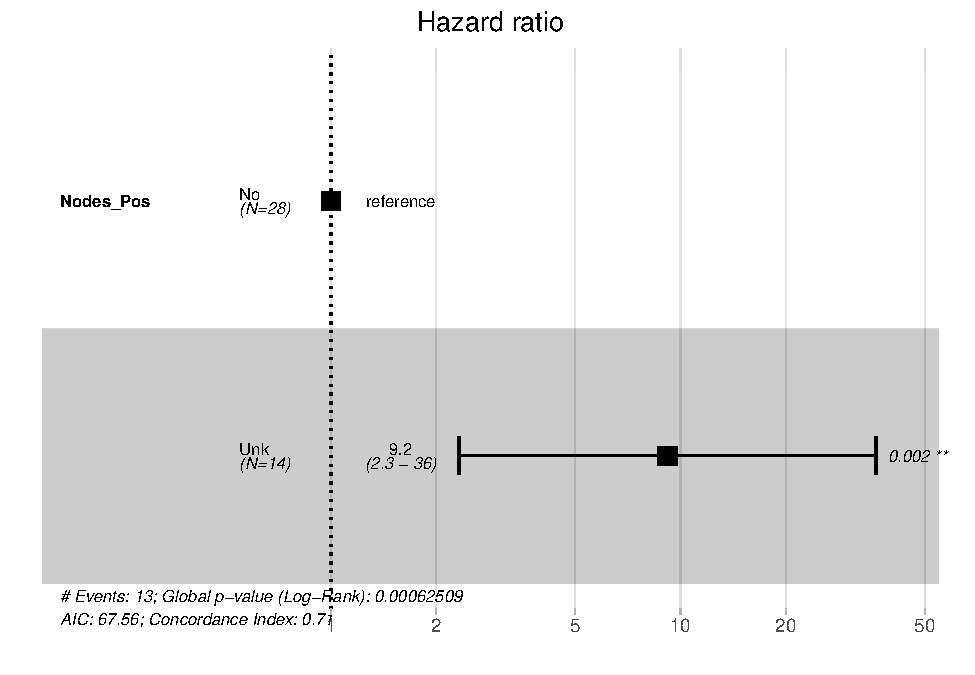
\includegraphics{EarlyOvaryByRace_files/figure-latex/unnamed-chunk-9-1.pdf}

\hypertarget{t1nxm0}{%
\paragraph{T1NxM0}\label{t1nxm0}}

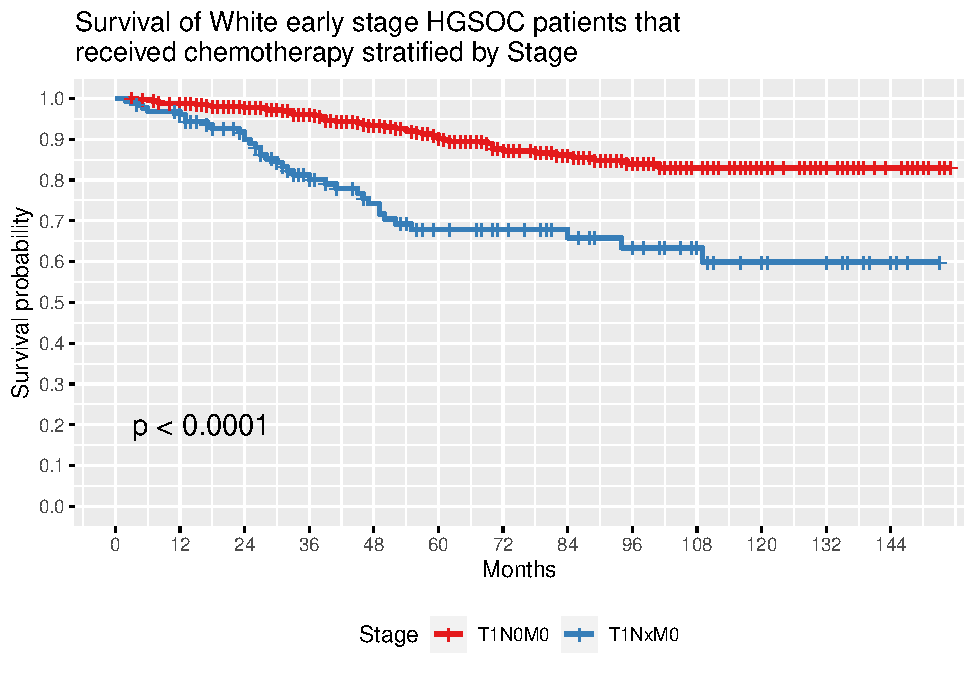
\includegraphics{EarlyOvaryByRace_files/figure-latex/unnamed-chunk-10-1.pdf}

\begin{tabular}[t]{l|r|r}
\hline
\multicolumn{1}{c|}{Black Race} & \multicolumn{2}{c}{Chemo Received} \\
\cline{1-1} \cline{2-3}
  & No/Unknown & Yes\\
\hline
no & 94 & 163\\
\hline
yes & 3 & 14\\
\hline
\end{tabular}

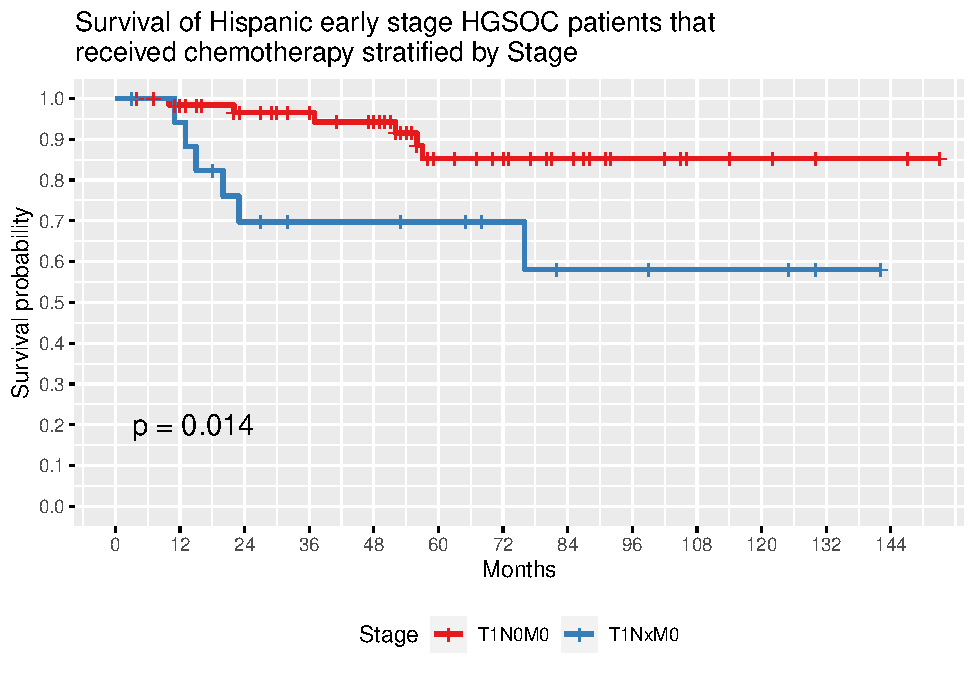
\includegraphics{EarlyOvaryByRace_files/figure-latex/unnamed-chunk-12-1.pdf}

\begin{Shaded}
\begin{Highlighting}[]
\KeywordTok{table}\NormalTok{(T1.Nx.M0.Black}\OperatorTok{$}\NormalTok{Black.Race, T1.Nx.M0.Black}\OperatorTok{$}\NormalTok{Chemo)}
\end{Highlighting}
\end{Shaded}

\begin{verbatim}
##      
##       No/Unknown Yes
##   no          94 163
##   yes          3  14
\end{verbatim}

\hypertarget{t1n1m0}{%
\paragraph{T1N1M0}\label{t1n1m0}}

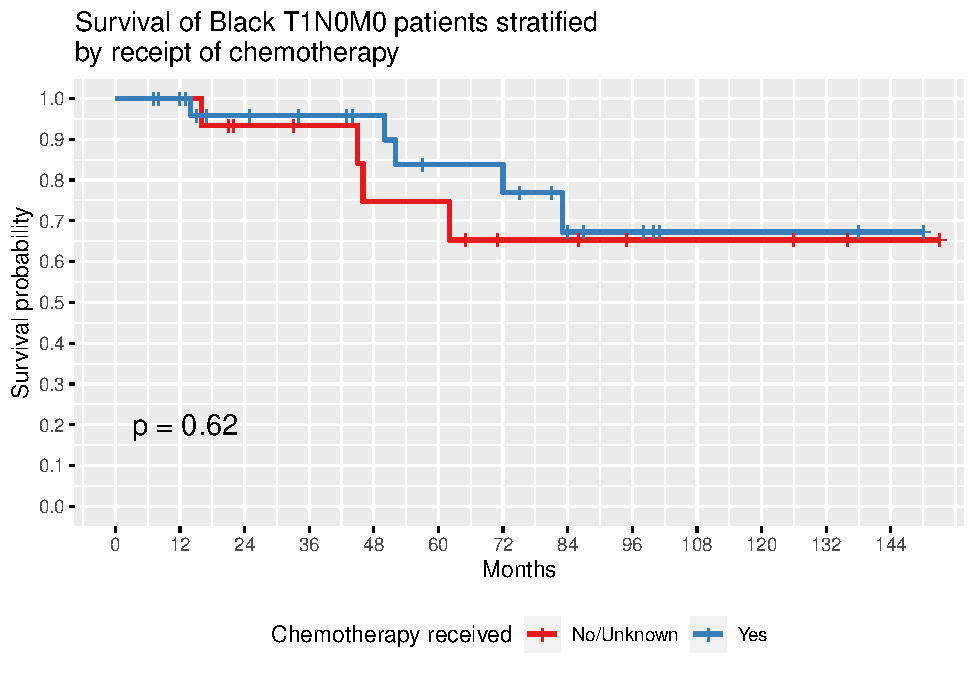
\includegraphics{EarlyOvaryByRace_files/figure-latex/unnamed-chunk-14-1.pdf}

\begin{Shaded}
\begin{Highlighting}[]
\KeywordTok{table}\NormalTok{(T1.N1.M0.Black}\OperatorTok{$}\NormalTok{Black.Race)}
\end{Highlighting}
\end{Shaded}

\begin{verbatim}
## 
##  no yes 
## 120  10
\end{verbatim}

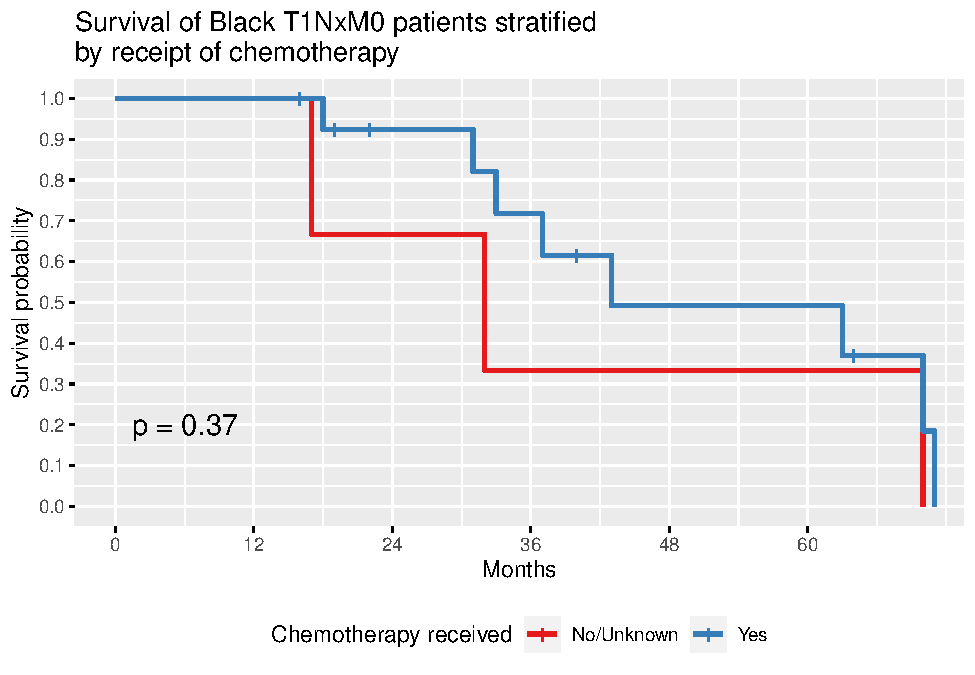
\includegraphics{EarlyOvaryByRace_files/figure-latex/unnamed-chunk-16-1.pdf}

\hypertarget{metastatic-disease}{%
\paragraph{Metastatic Disease}\label{metastatic-disease}}

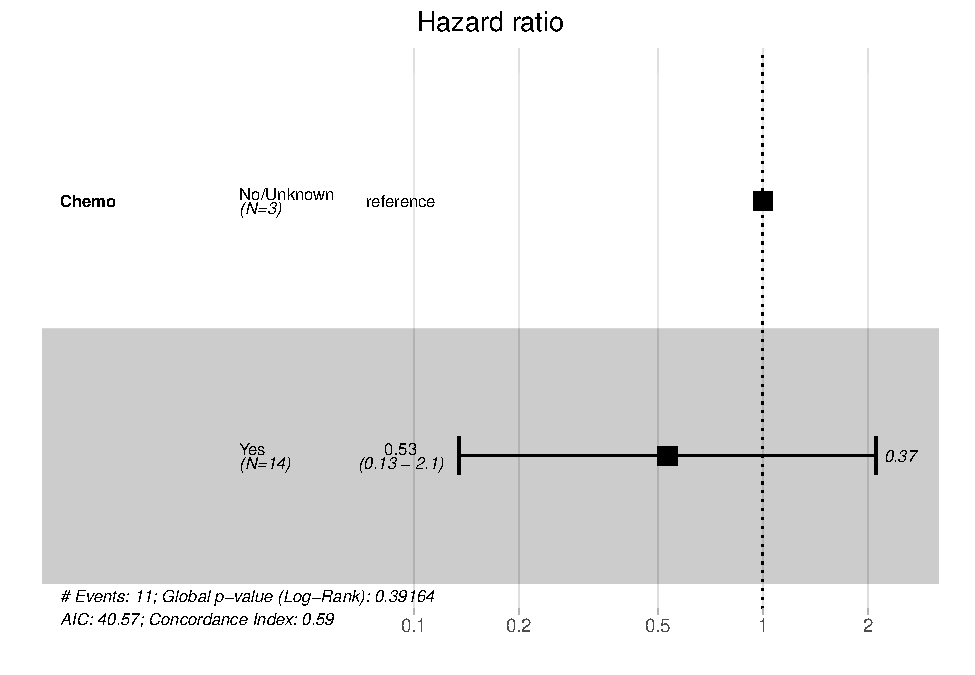
\includegraphics{EarlyOvaryByRace_files/figure-latex/unnamed-chunk-17-1.pdf}

\begin{Shaded}
\begin{Highlighting}[]
\KeywordTok{table}\NormalTok{(mets.Black}\OperatorTok{$}\NormalTok{Black.Race)}
\end{Highlighting}
\end{Shaded}

\begin{verbatim}
## 
##  no yes 
##  60   2
\end{verbatim}

\hypertarget{broken-down-by-whether-or-not-chemotherapy-was-received}{%
\subsubsection{Broken down by whether or not chemotherapy was
received}\label{broken-down-by-whether-or-not-chemotherapy-was-received}}

\hypertarget{with-chemotherapy}{%
\paragraph{With Chemotherapy}\label{with-chemotherapy}}

\includegraphics{EarlyOvaryByRace_files/figure-latex/unnamed-chunk-20-1.pdf}

\begin{Shaded}
\begin{Highlighting}[]
\KeywordTok{table}\NormalTok{(chemo.Black}\OperatorTok{$}\NormalTok{Black.Race)}
\end{Highlighting}
\end{Shaded}

\begin{verbatim}
## 
##  no yes 
## 880  50
\end{verbatim}

\hypertarget{without-chemotherapy}{%
\paragraph{Without Chemotherapy}\label{without-chemotherapy}}

\includegraphics{EarlyOvaryByRace_files/figure-latex/unnamed-chunk-22-1.pdf}

\begin{Shaded}
\begin{Highlighting}[]
\KeywordTok{table}\NormalTok{(nochemo.Black}\OperatorTok{$}\NormalTok{Black.Race)}
\end{Highlighting}
\end{Shaded}

\begin{verbatim}
## 
##  no yes 
## 317  23
\end{verbatim}

\hypertarget{comparing-only-black-race-to-white-race}{%
\subsection{Comparing only Black Race to White
Race}\label{comparing-only-black-race-to-white-race}}

\includegraphics{EarlyOvaryByRace_files/figure-latex/unnamed-chunk-24-1.pdf}

\begin{Shaded}
\begin{Highlighting}[]
\KeywordTok{table}\NormalTok{(HGS.White.Black}\OperatorTok{$}\NormalTok{Race.Group)}
\end{Highlighting}
\end{Shaded}

\begin{verbatim}
## 
## Black White 
##    73   956
\end{verbatim}

\hypertarget{broken-down-by-stage-1}{%
\subsubsection{Broken down by Stage}\label{broken-down-by-stage-1}}

\hypertarget{t1n0m0-1}{%
\paragraph{T1N0M0}\label{t1n0m0-1}}

\includegraphics{EarlyOvaryByRace_files/figure-latex/unnamed-chunk-27-1.pdf}

\begin{Shaded}
\begin{Highlighting}[]
\KeywordTok{table}\NormalTok{(T1.N0.M0}\OperatorTok{$}\NormalTok{Race.Group)}
\end{Highlighting}
\end{Shaded}

\begin{verbatim}
## 
## Black White 
##    43   601
\end{verbatim}

\hypertarget{t1nxm0-1}{%
\paragraph{T1NxM0}\label{t1nxm0-1}}

\includegraphics{EarlyOvaryByRace_files/figure-latex/unnamed-chunk-29-1.pdf}

\begin{Shaded}
\begin{Highlighting}[]
\KeywordTok{table}\NormalTok{(T1.Nx.M0}\OperatorTok{$}\NormalTok{Race.Group)}
\end{Highlighting}
\end{Shaded}

\begin{verbatim}
## 
## Black White 
##    17   206
\end{verbatim}

\hypertarget{t1n1m0-1}{%
\paragraph{T1N1M0}\label{t1n1m0-1}}

\includegraphics{EarlyOvaryByRace_files/figure-latex/unnamed-chunk-31-1.pdf}

\begin{Shaded}
\begin{Highlighting}[]
\KeywordTok{table}\NormalTok{(T1.N1.M0}\OperatorTok{$}\NormalTok{Race.Group)}
\end{Highlighting}
\end{Shaded}

\begin{verbatim}
## 
## Black White 
##    10    94
\end{verbatim}

\hypertarget{metastatic-disease-1}{%
\paragraph{Metastatic Disease}\label{metastatic-disease-1}}

\includegraphics{EarlyOvaryByRace_files/figure-latex/unnamed-chunk-33-1.pdf}

\begin{Shaded}
\begin{Highlighting}[]
\KeywordTok{table}\NormalTok{(mets}\OperatorTok{$}\NormalTok{Race.Group)}
\end{Highlighting}
\end{Shaded}

\begin{verbatim}
## 
## Black White 
##     2    49
\end{verbatim}

\hypertarget{broken-down-by-whether-or-not-chemotherapy-was-received-1}{%
\subsubsection{Broken down by whether or not chemotherapy was
received}\label{broken-down-by-whether-or-not-chemotherapy-was-received-1}}

\hypertarget{with-chemotherapy-1}{%
\paragraph{With Chemotherapy}\label{with-chemotherapy-1}}

\includegraphics{EarlyOvaryByRace_files/figure-latex/unnamed-chunk-36-1.pdf}

\begin{Shaded}
\begin{Highlighting}[]
\KeywordTok{table}\NormalTok{(chemo}\OperatorTok{$}\NormalTok{Race.Group)}
\end{Highlighting}
\end{Shaded}

\begin{verbatim}
## 
## Black White 
##    50   712
\end{verbatim}

\hypertarget{without-chemotherapy-1}{%
\paragraph{Without Chemotherapy}\label{without-chemotherapy-1}}

\includegraphics{EarlyOvaryByRace_files/figure-latex/unnamed-chunk-38-1.pdf}

\begin{Shaded}
\begin{Highlighting}[]
\KeywordTok{table}\NormalTok{(nochemo}\OperatorTok{$}\NormalTok{Race.Group)}
\end{Highlighting}
\end{Shaded}

\begin{verbatim}
## 
## Black White 
##    23   244
\end{verbatim}

\end{document}
